
\begin{frame}
    \frametitle{Problem Set 3.4 - 7 --- Pushkar Mohile}
    \emph{Problem Statement}\\
    Show that the discrete and indiscrete topologies on a
    set give rise to functors

\begin{equation*}
    \cat{Set}\to \cat{Top}
\end{equation*}    
    
    and these are the left and right adjoints, respectively, to the forgetful
    functor from Top to Set. 
\end{frame}
\begin{frame}
    
Solution : 

We begin by recalling the definition of a functor. Given two categories
\(\textsf{C}\) and \(\textsf{D}\), a functor \(\mathcal{F} \) assigns to every
object \(a \text{ in } \textsf{C}\) an object \(\mathcal{F}(a)\text{ in }\textsf{D}\), and for
every morphism \(f \in C(a,b)\) a corresponding morphism 
\begin{equation}
\mathcal{F}(f) \in \text{D}(\mathcal{F}(a), \mathcal{F}(b) )
\end{equation}
which respects composition 
\begin{equation}
    \mathcal{F}(f\circ g) = \mathcal{F}(f) \circ \mathcal{F}(g)
\end{equation}
    and maps \(\textsf{id} \text{ to } \textsf{id}\).

    \begin{center}
        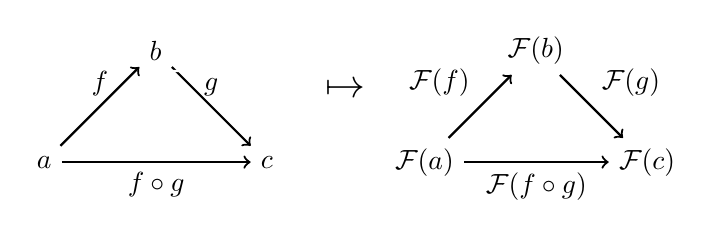
\begin{tikzpicture}[node distance={2cm}, thick, main/.style = {draw=none}]
            \node[main] (1)                         {\(b\)};
            \node[main] (2) [below left of=1]       {\(a\)};
            \node[main] (3) [below right of=1]      {\(c\)};

            \node[main] (4) [right of=3]            {\(\mathcal{F}(a)\)};
            \node[main] (5) [above right of=4]      {\(\mathcal{F}(b)\)};
            \node[main] (6) [below right of=5]      {\(\mathcal{F}(c)\)};
            
            \draw[->] (2) to node[midway, above] {\(f\)} (1);
            \draw[->] (1) to node[midway, above] {\(g\)} (3);
            \draw[->] (2) to node[midway, below] {\(f\circ g\)} (3);

            \draw[->, color=white] (1.south) to node[midway, below] {\Large\textcolor{black}{\(\mapsto\)}} (5.south) ; 
                
            \draw[->] (4) to node[midway, above left] {\(\mathcal{F}(f)\)} (5);
            \draw[->] (5) to node[midway, above right] {\(\mathcal{F}(g)\)} (6);
            \draw[->] (4) to node[midway, below] {\(\mathcal{F}(f\circ g)\)} (6);
        \end{tikzpicture}
    \end{center}

\end{frame}

\begin{frame}
    
Let us construct the functors corresponding to the discrete and indiscrete
topologies on any set \(X\) given by \(\tau_{disc} = 2^X\) and \(\tau_{indisc} =
\{\emptyset,X \}\). We will call them \textit{disc}: \(\textsf{Set} \to
\textsf{Top}\) and \textit{indisc}: \(\textsf{Set}\to \textsf{Top}\) , defined
in the following way 

\begin{gather*}
    \textit{disc}(X) \mapsto (X, \tau_{disc}) \\
    \textit{indisc}(X) \mapsto (X,\tau_{indisc}) 
\end{gather*}
And for any function \(f \in \textsf{Set}(X,Y)\), \(f:X\to Y\mapsto f:(X,
\tau_{disc})\to(Y,\tau_{disc})\) for \(disc\) \\ \(f:X\to Y\mapsto f:(X,
\tau_{indisc})\to(Y,\tau_{indisc})\) for \(indisc\) .
% Rewrite this later . Check Swapneel's way of writing this and write in the
% same style. 
\\ \pause
The check we need to make here is that \(f\) is a continuous function between
sets with the discrete and indiscrete topologies. 
\end{frame}

\begin{frame}
    
 For the discrete topology, this is done by noting that 
 
 \begin{equation}
    \forall \textnormal{ open sets } U \in \tau_Y , f^{-1} (U) \subseteq X \implies f^{-1} (U)\in 2^X
 \end{equation}

    and hence \(f^{-1}(U)\) is open in \(\tau_{disc}\). 

    % add some stuff for discrete topology
    % split indiscrete to another slide
\end{frame}
\begin{frame}
  Similarly, for the indiscrete topology, the only open subsets of \(Y\) are
    \({\emptyset,Y}\).  \\ For \(\emptyset \in \tau_Y\) we have
    \(f^{-1}(\emptyset) = \emptyset \in \tau_X \) and \(f^{-1}(Y) = X \cup
    \emptyset \in \tau_X \)  %\note{Clarify}
and hence once again \(f\) is continuous. \\The composition law is valid since
composition of continuous functions are continuous. Hence the discrete and
indiscrete topologies define the required functors. 

\end{frame}

\begin{frame}
    
For the second part, we have to show that these are left adjoint and right
adjoints respectively to the forgetful functor defined as follows: 
\begin{gather*}
    frg : \textsf{Top} \to \textsf{Set} \\
    (X, \tau_X ) \mapsto X \\
    f \in \textsf{Top}((X,\tau_X),(Y,\tau_Y )) \mapsto f \in \textsf{Set}(X,Y) 
\end{gather*}
i.e. we are forgetting the underlying topology and viewing the function \(f\) as a
morphism between sets. 
\end{frame}
\begin{frame}

    \begin{center}
        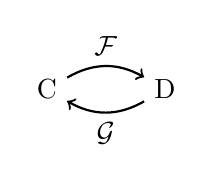
\begin{tikzpicture}[node distance={1.5cm}, thick, main/.style = {draw=none}]
            \node[main] (1)                         {C};
            \node[main] (2) [right of=1]            {D};
            
            \draw[->] (1) [bend right=-30] to node[midway, above] {\(\mathcal{F}\)} (2);
            \draw[->] (2) [bend left=30] to node[midway, below] {\(\mathcal{G}\)} (1);
        \end{tikzpicture}
    \end{center}
    
We recall the definitions of left and right adjoint functors. Given two
categories \(\textsf{C}\) and \(\textsf{D}\) and functors \(\mathcal{F}:
\textsf{C} \to \textsf{D}\) and \(\mathcal{G}: \textsf{D} \to \textsf{C}\), we
say that \(\mathcal{F}\) is a left adjoint and \(\mathcal{G}\) is a right
adjoint if for each object \(a \in\) \textsf{C} and \(x \in\textsf{D}\) , there
is a bijection between the sets of morphisms 

\begin{gather*}
    \textsf{D}(\mathcal{F}(a) , x) \xrightarrow{\cong} \textsf{C}(a,
    \mathcal{G}(x))
\end{gather*}

that is \textit{natural} in \(a\) and \(x\). 
\end{frame}
\begin{frame}
The naturality condition is
formally stated as follows: For any morphism \(a \to a'\) in \textsf{C} and \(x
\to x'\) in \textsf{D}, we have the following commutative diagrams (Check Cat
Theory lec. 2 or section 4.3 of the cat theory notes ) % subtle advertisement
% comment that this essentially implies it is independent of a and x
% add comment about Vec and Set if possible as a recognizable example
    \begin{center}
        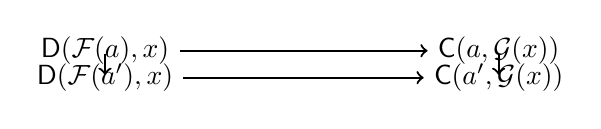
\begin{tikzpicture}[node distance={5cm}, thick, main/.style = {draw=none}]
            \node[main] (1)                 {\(\textsf{D}(\mathcal{F}(a), x)\)};
            \node[main] (2) [right of=1]    {\(\textsf{C}(a, \mathcal{G}(x))\)};
            \node[main] (3) [below=1]       {\(\textsf{D}(\mathcal{F}(a'), x)\)};        
            \node[main] (4) [right of=3]    {\(\textsf{C}(a', \mathcal{G}(x))\)};
            
            \draw[->] (1) to (2);
            \draw[->] (3) to (1);
            \draw[->] (3) to (4);
            \draw[->] (4) to (2);
        \end{tikzpicture}
    \end{center}
\end{frame}

\begin{frame}

    And, the naturality condition for \(x \to x'\) gives us the following
    commutative diagram:

    \begin{center}
        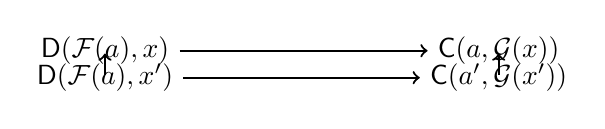
\begin{tikzpicture}[node distance={5cm}, thick, main/.style = {draw=none}]
            \node[main] (1)                 {\(\textsf{D}(\mathcal{F}(a), x)\)};
            \node[main] (2) [right of=1]    {\(\textsf{C}(a, \mathcal{G}(x))\)};
            \node[main] (3) [below=1]       {\(\textsf{D}(\mathcal{F}(a), x')\)};        
            \node[main] (4) [right of=3]    {\(\textsf{C}(a', \mathcal{G}(x'))\)};
            
            \draw[->] (1) to (2);
            \draw[->] (1) to (3);
            \draw[->] (3) to (4);
            \draw[->] (2) to (4);
        \end{tikzpicture}
    \end{center}

\end{frame}

\begin{frame}

    \begin{center}
        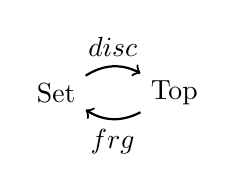
\begin{tikzpicture}[node distance={1.5cm}, thick, main/.style = {draw=none}]
            \node[main] (1)                         {Set};
            \node[main] (2) [right of=1]            {Top};
            
            \draw[->] (1) [bend right=-30] to node[midway, above] {\(disc\)} (2);
            \draw[->] (2) [bend left=30] to node[midway, below] {\(frg\)} (1);
        \end{tikzpicture}
    \end{center}
    
We now check the adjuction between \(frg\) and \(disc\) as  defined previously.
Let \(X \) be any set and \((Y,\tau_Y)\) be any topological space. We have to
prove that 
\begin{equation}
    \cat{Top}(\textit{disc}(X) , (Y, \tau_Y)  ) \bijec \cat{Set}(X, Y)
\end{equation}

\pause

This bijection is given by  \(f \mapsto f \) in both directions. We now have to
simply check whether the two sets are the same. This is done as follows: 
\begin{equation}
    \cat{Top}(\textit{disc}(X) , (Y, \tau_Y)  ) \subseteq \cat{Set}(X, Y)
\end{equation}
is obvious since continuous functions are functions between the sets. 
\end{frame}
\begin{frame}
    
Next, note that 
\begin{equation}
    \cat{Set}(X, Y) \subseteq \cat{Top}(\textit{disc}(X) , (Y, \tau_Y)  )
\end{equation}

    Let \(f \in \cat{Set}(X,Y)\),  \(U_Y\) be any open set in \(\tau_Y\).
    \(f^{-1}(U) \subseteq X \in 2^X\) and hence \(f\) is continuous. \\
    Thus we have proved that the two sets of morphisms are equal. Finally we make note of the
    naturality condition. 
    % explain this more clearly
\end{frame}
\begin{frame}

    Given \(h \in Set(X, X')\) and \(j \in Top((Y,\tau_Y), (Y',\tau_{Y'}))\),
    
    \begin{center}
        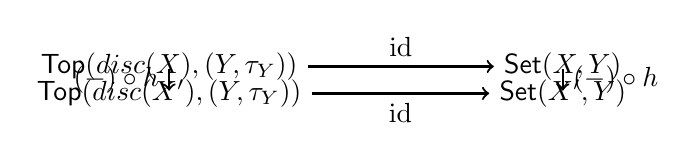
\begin{tikzpicture}[node distance={5cm}, thick, main/.style = {draw=none}]
            \node[main] (1)                 {\(\textsf{Top}(disc(X), (Y,\tau_Y))\)};
            \node[main] (2) [right of=1]    {\(\textsf{Set}(X, Y)\)};
            \node[main] (3) [below=1]       {\(\textsf{Top}(disc(X'), (Y,\tau_Y))\)};        
            \node[main] (4) [right of=3]    {\(\textsf{Set}(X', Y)\)};
            
            \draw[->] (1) to node [midway, above] {id} (2);
            \draw[->] (3) to node [midway, left] {\((-)\circ h\)} (1);
            \draw[->] (3) to node [midway, below] {id} (4);
            \draw[->] (4) to node [midway, right] {\((-)\circ h\)} (2);
        \end{tikzpicture}
        \\ \phantom{1}\\ \pause
        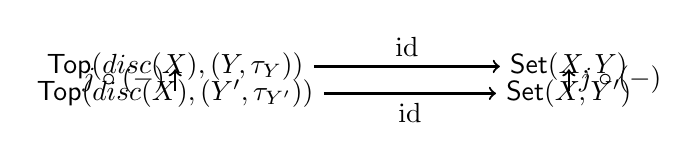
\begin{tikzpicture}[node distance={5cm}, thick, main/.style = {draw=none}]
            \node[main] (1)                 {\(\textsf{Top}(disc(X), (Y,\tau_Y))\)};
            \node[main] (2) [right of=1]    {\(\textsf{Set}(X, Y)\)};
            \node[main] (3) [below=1]       {\(\textsf{Top}(disc(X), (Y',\tau_{Y'}))\)};        
            \node[main] (4) [right of=3]    {\(\textsf{Set}(X, Y')\)};
            
            \draw[->] (1) to node [midway, above] {id} (2);
            \draw[->] (1) to node [midway, left] {\(j \circ (-)\)} (3);
            \draw[->] (3) to node [midway, below] {id} (4);
            \draw[->] (2) to node [midway, right] {\(j \circ (-)\)} (4);
        \end{tikzpicture}
    \end{center}    

\end{frame}

\begin{frame}
    
This adjunction can be restated in terms of the following universal property of
the discrete topology : The discrete topology on \(X\) is the topology such that
every function from \(X\) to any topological space \( (Y, \tau_Y)\) is continuous. 
%Draw diagram


\begin{center}
    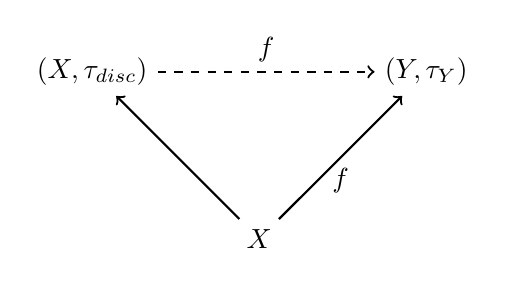
\begin{tikzpicture}[node distance={3cm}, thick, main/.style = {draw=none}]
        \node[main] (1)                         {\(X\)};
        \node[main] (2) [above left of=1]            {\((X, \tau_{disc})\)};
        \node[main] (3) [above right of=1]            {\((Y, \tau_Y)\)};
        
        \draw[->] (1) to (2);
        \draw[->] (1) to node[midway, below] {\(f\)} (3);
        \draw[->] (2) to node[midway, above] {\(f\)} (3) [dashed];
    \end{tikzpicture}
\end{center}


\end{frame}

\begin{frame}

    \begin{center}
        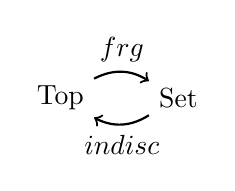
\begin{tikzpicture}[node distance={1.5cm}, thick, main/.style = {draw=none}]
            \node[main] (1)                         {Set};
            \node[main] (2) [left of=1]            {Top};
            
            \draw[->] (1) [bend right=-30] to node[midway, below] {\(indisc\)} (2);
            \draw[->] (2) [bend left=30] to node[midway, above] {\(frg\)} (1);
        \end{tikzpicture}
    \end{center}

    Finally we take a look at the right adjoint condition for the indiscrete
    topology. The condition states that 
    \begin{equation}
         \cat{Set}(Y,X ) \bijec \cat{Top}((Y, \tau_Y) ,\textit{indisc}(X))
    \end{equation}
    The checks are similar to the previously done checks.

\end{frame}

\begin{frame}

    We mention the only nontrivial check: 
    \begin{equation}
        \cat{Set}(Y,X ) \subseteq\cat{Top}((Y, \tau_Y) ,\textit{indisc}(X))
    \end{equation}

    For a given function \(f \in   \cat{Set}(Y,X )\), with the indiscrete
    topology on \(X\), \(f^{-1}(\emptyset) = \emptyset\) and \(f^{-1}(X) = Y
    \cup \emptyset\), both of which are open wrt any topology on \(Y\). Hence
    \(f\) is continuous. 

    What is the universal property? 

\end{frame}
